\documentclass[12pt,a4paper]{article}
\usepackage[utf8]{inputenc}
\usepackage[spanish]{babel}
\usepackage{amsmath}
\usepackage{amsfonts}
\usepackage{amssymb}
\usepackage{graphicx}
\usepackage[left=2.5cm,right=2.5cm,top=3cm,bottom=3cm]{geometry}
\usepackage{xcolor}
\usepackage{listings}
\usepackage{tcolorbox}
\usepackage{hyperref}

% Configuración de colores para código
\definecolor{codegreen}{rgb}{0,0.6,0}
\definecolor{codegray}{rgb}{0.5,0.5,0.5}
\definecolor{codepurple}{rgb}{0.58,0,0.82}
\definecolor{backcolour}{rgb}{0.95,0.95,0.92}

\lstdefinestyle{mystyle}{
    backgroundcolor=\color{backcolour},   
    commentstyle=\color{codegreen},
    keywordstyle=\color{magenta},
    numberstyle=\tiny\color{codegray},
    stringstyle=\color{codepurple},
    basicstyle=\ttfamily\footnotesize,
    breakatwhitespace=false,         
    breaklines=true,                 
    captionpos=b,                    
    keepspaces=true,                 
    numbers=left,                    
    numbersep=5pt,                  
    showspaces=false,                
    showstringspaces=false,
    showtabs=false,                  
    tabsize=2
}
\lstset{style=mystyle}

\title{\textbf{Guía de Laboratorio 4}\\ \Large Detector de Distancia Ultrasónico}
\author{Andrés}
\date{\today}

\begin{document}

\maketitle

\section{Introducción}
En este proyecto se construye un medidor de distancia digital utilizando un sensor ultrasónico HC-SR04 y una placa Arduino. El sistema mide el tiempo que tarda una onda sonora en rebotar contra un objeto y calcula la distancia basándose en la velocidad del sonido. Los resultados se muestran en tiempo real en una pantalla LCD I2C.

\section{Materiales y Ensamblaje del Circuito}
\begin{itemize}
    \item Placa Arduino Uno
    \item Sensor Ultrasónico HC-SR04
    \item Pantalla LCD 16x2 con Módulo I2C
    \item Protoboard y Jumpers
\end{itemize}

\begin{tcolorbox}[colback=teal!5!white,colframe=teal!75!black,title=Detalle de Pines]
\textbf{Sensor HC-SR04:} VCC a 5V, GND a GND, Trig al Pin 9, Echo al Pin 10.\\
\textbf{Pantalla LCD I2C:} VCC a 5V, GND a GND, SDA al pin A4, SCL al pin A5.
\end{tcolorbox}

\begin{figure}[h]
    \centering
    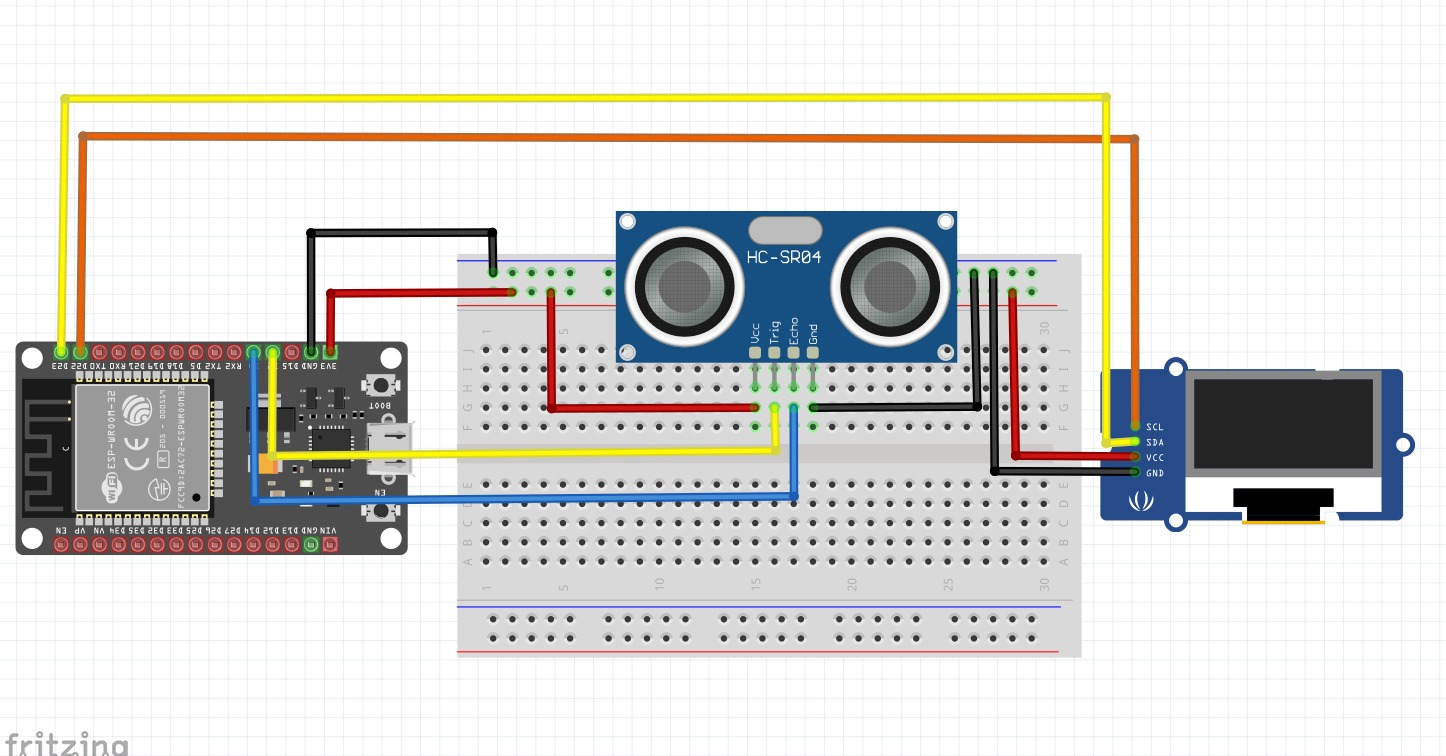
\includegraphics[width=0.7\textwidth]{circuito_distancia.jpeg}
    \caption{Diagrama de conexiones del sensor de distancia.}
\end{figure}

\subsection{Fotos del Ensamblaje Real}
\begin{figure}[h]
    \centering
    \begin{minipage}{0.48\textwidth}
        \centering
        \includegraphics[width=\textwidth]{"detector de distancia/WhatsApp Image 2026-05-15 at 12.49.25 PM (1).jpeg"}
        \caption{Conexión del sensor ultrasónico.}
    \end{minipage}
    \hfill
    \begin{minipage}{0.48\textwidth}
        \centering
        \includegraphics[width=\textwidth]{"detector de distancia/WhatsApp Image 2026-05-15 at 12.49.25 PM (2).jpeg"}
        \caption{Montaje final en protoboard.}
    \end{minipage}
\end{figure}

\section{Código Fuente}
\begin{lstlisting}[language=C++]
#include <Wire.h>
#include <LiquidCrystal_I2C.h>

// Definicion de pines para el sensor HC-SR04
const int TrigPin = 9;
const int EchoPin = 10;

long duracion;
int distancia;

LiquidCrystal_I2C lcd(0x27, 16, 2);

void setup() {
  pinMode(TrigPin, OUTPUT);
  pinMode(EchoPin, INPUT);
  
  lcd.init();
  lcd.backlight();
  lcd.setCursor(0, 0);
  lcd.print("Medidor de Dist.");
  delay(2000);
  lcd.clear();
}

void loop() {
  // Limpiar el TrigPin
  digitalWrite(TrigPin, LOW);
  delayMicroseconds(2);
  
  // Activar el sensor por 10 microsegundos
  digitalWrite(TrigPin, HIGH);
  delayMicroseconds(10);
  digitalWrite(TrigPin, LOW);
  
  // Leer el EchoPin (tiempo de rebote en microsegundos)
  duracion = pulseIn(EchoPin, HIGH);
  
  // Calcular distancia (Vel. sonido = 340 m/s o 0.034 cm/us)
  // Distancia = (Tiempo * Velocidad) / 2
  distancia = duracion * 0.034 / 2;
  
  // Mostrar en LCD
  lcd.setCursor(0, 0);
  lcd.print("Distancia:");
  lcd.setCursor(0, 1);
  lcd.print(distancia);
  lcd.print(" cm          ");
  
  delay(500);
}
\end{lstlisting}

\section{Pruebas y Resultados}
\begin{enumerate}
    \item Coloca el sensor HC-SR04 de frente a una superficie plana.
    \item Mueve la superficie hacia adelante y atrás.
    \item Verifica que la lectura en la pantalla LCD cambie con precisión según el movimiento.
\end{enumerate}

\begin{figure}[h]
    \centering
    \setlength{\fboxsep}{10pt}
    \setlength{\fboxrule}{1pt}
    \fbox{\rule{0pt}{100pt} \parbox{0.8\textwidth}{\centering \textit{Espacio para fotografía del circuito en funcionamiento}}}
    \caption{Medidor de distancia en operación.}
\end{figure}

\end{document}

